\chapter{Advanced Automation Strategies}

\section{Introduction}

As you become more proficient with basic automation techniques, it's time to explore advanced strategies that can set your IT consulting practice apart. In this chapter, we'll delve into integrating AI and machine learning, implementing automated testing and deployment, and building reusable components to accelerate your projects.

\section{Integrating AI and Machine Learning into Your Workflow}

Artificial Intelligence (AI) and Machine Learning (ML) are no longer just buzzwords - they're powerful tools that can significantly enhance your automation workflows. Let's explore how you can leverage these technologies using no-code tools.

\subsection{Leveraging LangChain in n8n}

LangChain is a framework for developing applications powered by language models. When integrated with n8n, it opens up a world of possibilities for natural language processing in your workflows.

Here's how you can use LangChain in n8n:

1. \textbf{Text Summarization}:
\begin{itemize}
    \item Use LangChain to automatically summarize lengthy documents or emails
    \item Implement in client communication workflows to quickly extract key points
\end{itemize}

% TODO @screenshot: n8n workflow using LangChain for text summarization

% TODO @qr: QR code for downloading the text summarization n8n workflow sample

2. \textbf{Sentiment Analysis}:
\begin{itemize}
    \item Analyze customer feedback or support tickets to gauge sentiment
    \item Trigger appropriate workflows based on positive or negative sentiment
\end{itemize}

% TODO @qr: QR code for downloading the sentiment analysis n8n workflow sample

3. \textbf{Automated Content Generation}:
\begin{itemize}
    \item Generate draft responses to common client inquiries
    \item Create initial project proposals based on client requirements
\end{itemize}

% TODO @qr: QR code for downloading the automated content generation n8n workflow sample

\subsection{Implementing AI-Powered Decision Making}

Use AI to enhance your decision-making processes:

1. \textbf{Predictive Maintenance}:
\begin{itemize}
    \item Implement ML models to predict when client systems may need maintenance
    \item Use n8n to trigger alerts or create maintenance tickets automatically
\end{itemize}

2. \textbf{Anomaly Detection}:
\begin{itemize}
    \item Monitor client systems for unusual patterns or behaviors
    \item Automatically escalate potential security threats or performance issues
\end{itemize}

\begin{tikzpicture}[node distance=2cm, auto]
        % Define styles
    \tikzstyle{decision} = [diamond, draw, fill=blue!20,
    text width=4.5em, text badly centered, node distance=3cm, inner sep=0pt]
    \tikzstyle{block} = [rectangle, draw, fill=blue!20,
    text width=5em, text centered, rounded corners, minimum height=4em]
    \tikzstyle{line} = [draw, -latex']

    % Place nodes
    \node [block] (input) {Input Data};
    \node [block, right of=input, node distance=4cm] (preprocess) {Preprocess Data};
    \node [block, right of=preprocess, node distance=4cm] (aimodel) {AI Model};
    \node [decision, below of=aimodel] (decide) {Decision};
    \node [block, left of=decide, node distance=4cm] (action1) {Action 1};
    \node [block, right of=decide, node distance=4cm] (action2) {Action 2};
    \node [block, below of=decide, node distance=3cm] (feedback) {Feedback Loop};

    % Draw edges
    \path [line] (input) -- (preprocess);
    \path [line] (preprocess) -- (aimodel);
    \path [line] (aimodel) -- (decide);
    \path [line] (decide) -- node [near start] {Yes} (action1);
    \path [line] (decide) -- node [near start] {No}  (action2);
    \path [line] (action1) |- (feedback);
    \path [line] (action2) |- (feedback);
    \path [line] (feedback) -| (input);
\end{tikzpicture}

\subsection{Upselling AI Solutions to Clients}

Position your AI-enhanced services as a cost-effective alternative to in-house AI development:

1. \textbf{Demonstrate Clear ROI}:
\begin{itemize}
    \item Create case studies showing time and cost savings from AI integration
    \item Develop an AI ROI calculator for potential clients
\end{itemize}

2. \textbf{Offer Tiered AI Services}:
\begin{itemize}
    \item Basic: Simple automation with AI-powered elements (e.g., text summarization)
    \item Advanced: Custom AI models for specific client needs
    \item Enterprise: Full AI integration across client systems
\end{itemize}

\begin{tikzpicture}[scale=0.8]
        % Define colors
    \definecolor{basiccolor}{RGB}{173,216,230}
    \definecolor{advancedcolor}{RGB}{144,238,144}
    \definecolor{enterprisecolor}{RGB}{255,192,203}

    % Define styles
    \tikzstyle{tier}=[rectangle, rounded corners, minimum width=5cm, minimum height=2cm, text width=4.5cm, align=center, font=\small\bfseries]
    \tikzstyle{feature}=[text width=4.5cm, align=left, font=\tiny]

    % Enterprise Tier
    \node[tier, fill=enterprisecolor] (enterprise) at (0,4) {Enterprise AI Services};
    \node[feature, below=0.1cm of enterprise] (enterprise_features) {
        \textbullet~Full AI integration\\
        \textbullet~Cross-system solutions\\
        \textbullet~Advanced analytics
    };

    % Advanced Tier
    \node[tier, fill=advancedcolor] (advanced) at (0,1.5) {Advanced AI Services};
    \node[feature, below=0.1cm of advanced] (advanced_features) {
        \textbullet~Custom AI models\\
        \textbullet~Specific client needs\\
        \textbullet~Enhanced automation
    };

    % Basic Tier
    \node[tier, fill=basiccolor] (basic) at (0,-1) {Basic AI Services};
    \node[feature, below=0.1cm of basic] (basic_features) {
        \textbullet~Simple automation\\
        \textbullet~AI-powered elements\\
        \textbullet~Text summarization
    };

    % Arrow and label
    \draw[-stealth, thick] (-3,-1.5) -- (-3,4.5);
    \node[rotate=90, anchor=south, font=\small\bfseries] at (-3.5,1.5) {Increasing Complexity and Value};
\end{tikzpicture}

\section{Automated Testing and Deployment for Non-Developers}

Implementing robust testing and deployment processes is crucial for delivering reliable solutions. Here's how you can achieve this using no-code and low-code tools.

\subsection{Automated Testing with n8n}

Leverage n8n to create comprehensive testing workflows:

1. \textbf{API Testing}:
\begin{itemize}
    \item Use HTTP Request nodes to test API endpoints
    \item Implement IF nodes to check response codes and payload content
\end{itemize}

2. \textbf{Data Validation}:
\begin{itemize}
    \item Create workflows to validate data in NoCoDB tables
    \item Use Function nodes to implement complex validation logic
\end{itemize}

3. \textbf{User Flow Testing}:
\begin{itemize}
    \item Simulate user interactions in BudiBase applications using n8n
    \item Automate form submissions and check results
\end{itemize}

% TODO @screenshot: n8n workflow for automated testing of a BudiBase application

\subsection{Continuous Integration with GitHub Actions}

Implement a CI/CD pipeline using GitHub Actions:

1. \textbf{Automated builds}:
\begin{itemize}
    \item Set up GitHub Actions to build your n8n workflows and BudiBase apps
    \item Trigger builds on every push to your repository
\end{itemize}

2. \textbf{Running Tests}:
\begin{itemize}
    \item Execute your n8n testing workflows as part of the CI process
    \item Implement BudiBase-specific tests using tools like Cypress
\end{itemize}

3. \textbf{Deployment}:
\begin{itemize}
    \item Use GitHub Actions to deploy successful builds to staging environments
    \item Implement manual approval steps for production deployments
\end{itemize}
\begin{tikzpicture}[node distance=2cm, auto]
        % Define styles
    \tikzstyle{process} = [rectangle, rounded corners, minimum width=3cm, minimum height=1cm, text centered, draw=black, fill=blue!20]
    \tikzstyle{decision} = [diamond, aspect=2, draw=black, fill=green!20, text width=4em, text badly centered, inner sep=0pt]
    \tikzstyle{arrow} = [thick,->,>=stealth]

    % Nodes
    \node [process] (push) {Git Push};
    \node [process, right of=push, xshift=3cm] (actions) {GitHub Actions};
    \node [process, below of=actions, yshift=-1cm] (build) {Build};
    \node [process, right of=build, xshift=3cm] (test) {Test};
    \node [decision, right of=test, xshift=3cm] (success) {Tests Pass?};
    \node [process, below of=success, yshift=-1.5cm] (deploy_staging) {Deploy to Staging};

    % n8n and BudiBase specific nodes
    \node [process, below of=build, yshift=-1.5cm] (n8n_build) {n8n Workflows};
    \node [process, right of=n8n_build, xshift=3cm] (budi_build) {BudiBase Apps};

    % Arrows
    \draw [arrow] (push) -- (actions);
    \draw [arrow] (actions) -- (build);
    \draw [arrow] (build) -- (test);
    \draw [arrow] (test) -- (success);
    \draw [arrow] (success) -- node[right] {Yes} (deploy_staging);
    \draw [arrow] (success) -| node[near start, above] {No} ([xshift=-1cm]build.north) |- (build);

    % n8n and BudiBase specific arrows
    \draw [arrow] (build) -- (n8n_build);
    \draw [arrow] (build) -- (budi_build);

    % Labels
    \node [text width=3cm, text centered, below of=n8n_build, yshift=-0.5cm] {n8n Workflows};
    \node [text width=3cm, text centered, below of=budi_build, yshift=-0.5cm] {BudiBase Apps};
\end{tikzpicture}

\subsection{Monitoring and Alerts}

Set up monitoring for your deployed solutions:

1. \textbf{Performance Monitoring}:
\begin{itemize}
    \item Use n8n to periodically check response times of key API endpoints
    \item Implement custom metrics in BudiBase applications
\end{itemize}

2. \textbf{Error Tracking}:
\begin{itemize}
    \item Set up error logging in n8n workflows and BudiBase apps
    \item Use n8n to aggregate and analyze error logs
\end{itemize}

3. \textbf{Automated Alerts}:
\begin{itemize}
    \item Configure n8n to send alerts via email or Slack for critical issues
    \item Implement escalation workflows for unresolved problems
\end{itemize}

% TODO @screenshot: n8n workflow for monitoring and alerting

\section{Building Reusable Components to Accelerate Future Projects}

Creating a library of reusable components can significantly speed up your project delivery. Here are some best practices for IT consultants:

\subsection{Identifying Reusable Patterns}

1. \textbf{Analyze Past Projects}:
\begin{itemize}
    \item Look for common workflows or functionalities across different clients
    \item Identify frequently used UI components in BudiBase applications
\end{itemize}

2. \textbf{Standardize Common Processes}:
\begin{itemize}
    \item Create template workflows for onboarding, reporting, invoicing, etc.
    \item Develop standardized data models for common entities (e.g., clients, projects)
\end{itemize}

\subsection{Developing a Component Library}

1. \textbf{n8n Workflow Templates}:
\begin{itemize}
    \item Create a repository of common n8n workflows (e.g., data synchronization, notifications)
    \item Document each template with clear instructions and customization points
\end{itemize}

2. \textbf{BudiBase Component Library}:
\begin{itemize}
    \item Develop a set of custom BudiBase components for common needs (e.g., advanced search, multi-step forms)
    \item Create design guidelines to ensure consistency across projects
\end{itemize}

3. \textbf{NoCoDB Schema Templates}:
\begin{itemize}
    \item Design reusable database schemas for common business objects
    \item Create template views and forms for standard data operations
\end{itemize}

% TODO @screenshot: Example of a reusable n8n workflow template

\subsection{Implementing a Component Management System}

1. \textbf{Version Control}:
\begin{itemize}
    \item Use Git to manage versions of your reusable components
    \item Implement a branching strategy for component development and maintenance
\end{itemize}

2. \textbf{Documentation}:
\begin{itemize}
    \item Create comprehensive documentation for each reusable component
    \item Include usage examples, customization options, and best practices
\end{itemize}

3. \textbf{Component Showcase}:
\begin{itemize}
    \item Develop a showcase application demonstrating your reusable components
    \item Use this as a sales tool to demonstrate your capabilities to potential clients
\end{itemize}

% TODO @screenshot: Component showcase application built with BudiBase

\section{Case Study: Accelerating Project Delivery with Advanced Automation}

Let's examine how an IT consulting firm used these advanced strategies to dramatically improve their project delivery:

\begin{itemize}
    \item Reduced project setup time by 70% using reusable components
    \item Decreased bug reports by 50% through automated testing
    \item Increased client satisfaction scores by 40% with AI-powered insights
    \item Improved profit margins by 25% due to faster project delivery
\end{itemize}

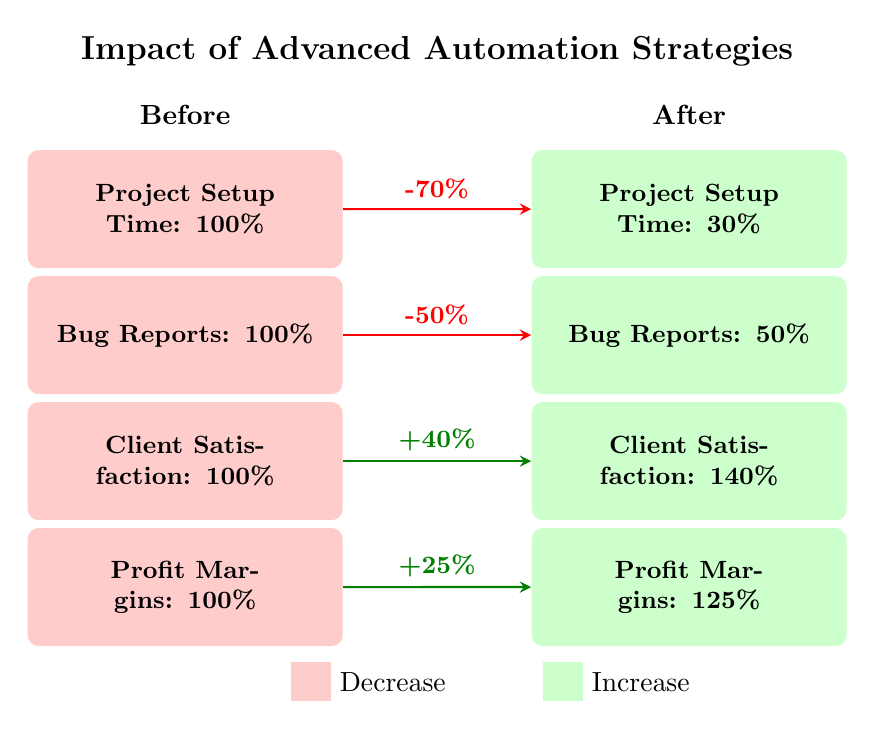
\begin{tikzpicture}[scale=0.8]
    % Define colors
    \definecolor{before}{RGB}{255,204,204}
    \definecolor{after}{RGB}{204,255,204}

    % Define styles
    \tikzstyle{stat} = [rectangle, rounded corners, minimum width=4cm, minimum height=1.5cm, text width=3.5cm, align=center, font=\small\bfseries]

    % Title
    \node[font=\large\bfseries] at (0,5.5) {Impact of Advanced Automation Strategies};

    % Before and After labels
    \node[font=\bfseries] at (-4,4.5) {Before};
    \node[font=\bfseries] at (4,4.5) {After};

    % Before column
    \node[stat, fill=before] (setup_before) at (-4,3) {Project Setup Time: 100\%};
    \node[stat, fill=before] (bugs_before) at (-4,1) {Bug Reports: 100\%};
    \node[stat, fill=before] (satisfaction_before) at (-4,-1) {Client Satisfaction: 100\%};
    \node[stat, fill=before] (profit_before) at (-4,-3) {Profit Margins: 100\%};

    % After column
    \node[stat, fill=after] (setup_after) at (4,3) {Project Setup Time: 30\%};
    \node[stat, fill=after] (bugs_after) at (4,1) {Bug Reports: 50\%};
    \node[stat, fill=after] (satisfaction_after) at (4,-1) {Client Satisfaction: 140\%};
    \node[stat, fill=after] (profit_after) at (4,-3) {Profit Margins: 125\%};

    % Arrows and labels
    \draw[-stealth, thick, red] (setup_before) -- (setup_after) node[midway, above, font=\small\bfseries] {-70\%};
    \draw[-stealth, thick, red] (bugs_before) -- (bugs_after) node[midway, above, font=\small\bfseries] {-50\%};
    \draw[-stealth, thick, green!50!black] (satisfaction_before) -- (satisfaction_after) node[midway, above, font=\small\bfseries] {+40\%};
    \draw[-stealth, thick, green!50!black] (profit_before) -- (profit_after) node[midway, above, font=\small\bfseries] {+25\%};

    % Legend
    \node[rectangle, fill=before, minimum size=0.5cm] at (-2,-4.5) {};
    \node[right] at (-1.7,-4.5) {Decrease};
    \node[rectangle, fill=after, minimum size=0.5cm] at (2,-4.5) {};
    \node[right] at (2.3,-4.5) {Increase};
\end{tikzpicture}

\section{Conclusion}

By implementing these advanced automation strategies - integrating AI, setting up robust testing and deployment processes, and building a library of reusable components - you can significantly enhance your IT consulting practice. These approaches not only improve your efficiency but also position you as a cutting-edge service provider capable of delivering sophisticated solutions rapidly.

\textbf{Action Items}:
\begin{enumerate}
    \item Experiment with integrating LangChain into one of your existing n8n workflows.
    \item Set up a basic CI/CD pipeline using GitHub Actions for one of your projects.
    \item Identify three common components from your recent projects and create reusable templates.
    \item Start building your component library and document your first reusable workflow.
\end{enumerate}

Remember, the key to success with these advanced strategies is continuous learning and iteration. Stay curious, keep experimenting, and always look for ways to improve your automation toolkit.

% TODO @qr: QR code linking to additional resources on advanced automation strategies